% \section{Methodology}
% \label{sec:method}

% \subsection{Objective and problem formulation}
% \label{sec:objective}

% We study supervised reasoning tasks where each training example consists of a question $q$,
% an optional chain-of-thought $r = (r_1,\dots,r_M)$, and a final answer
% $a = (a_1,\dots,a_N)$. The full textual sequence is
% \[
% y \;=\; [\,q \,;\, r \,;\, a\,].
% \]
% A standard causal language model (LM) parameterized by $\theta$ learns $p_\theta(y)$ via maximum
% likelihood training.

% \paragraph{Goal.}
% Our goal is to enable multi-step reasoning using \emph{continuous} internal representations while
% preserving standard autoregressive decoding of the answer, and crucially, avoiding the \emph{serial}
% compute bottleneck that arises when continuous reasoning is implemented through recurrent latent
% unrolling.

% \paragraph{Key bottleneck.}
% Chain of Continuous Thought (Coconut)~\cite{hao2024training} replaces segments of the textual rationale
% with continuous latent states, but generates these states \emph{sequentially} by feeding the previous
% hidden state back as the next input embedding. This induces a recurrent dependency across latent steps,
% causing serial depth to grow linearly with the number of latent states and limiting hardware
% parallelism and representational independence.

% \paragraph{Hypothesis.}
% We hypothesize that the benefits of continuous latent reasoning do not require recurrent latent
% unrolling. Instead, effective reasoning can be achieved by (i) synthesizing a \emph{set} of latent
% reasoning states in parallel from the current textual context, (ii) allowing structured interaction
% among these states, and (iii) conditioning autoregressive decoding on them through a causal interface.

% \subsection{Preliminaries: causal LMs and Coconut-style latent replacement}
% \label{sec:prelims}

% A causal Transformer LM maps token prefixes $x_{\le t}$ to hidden states
% $H_t \in \mathbb{R}^{t \times d}$ and predicts the next token via
% \[
% p_\theta(x_{t+1}\mid x_{\le t}) = \mathrm{softmax}(W h_t).
% \]

% Coconut~\cite{hao2024training} replaces a prefix of textual CoT tokens with continuous latent states that
% are not decoded as language. During this latent phase, each latent is generated by feeding the
% previous hidden state as the next input embedding, creating a recurrent unrolling within the
% Transformer. Although this enables latent reasoning, each additional latent step introduces an
% additional serial dependency and Transformer invocation, reinstating an RNN-like bottleneck.

% \subsection{Parallel Continuous Thought (PaCT)}
% \label{sec:pact}

% \begin{figure*}[t]
%   \centering
%   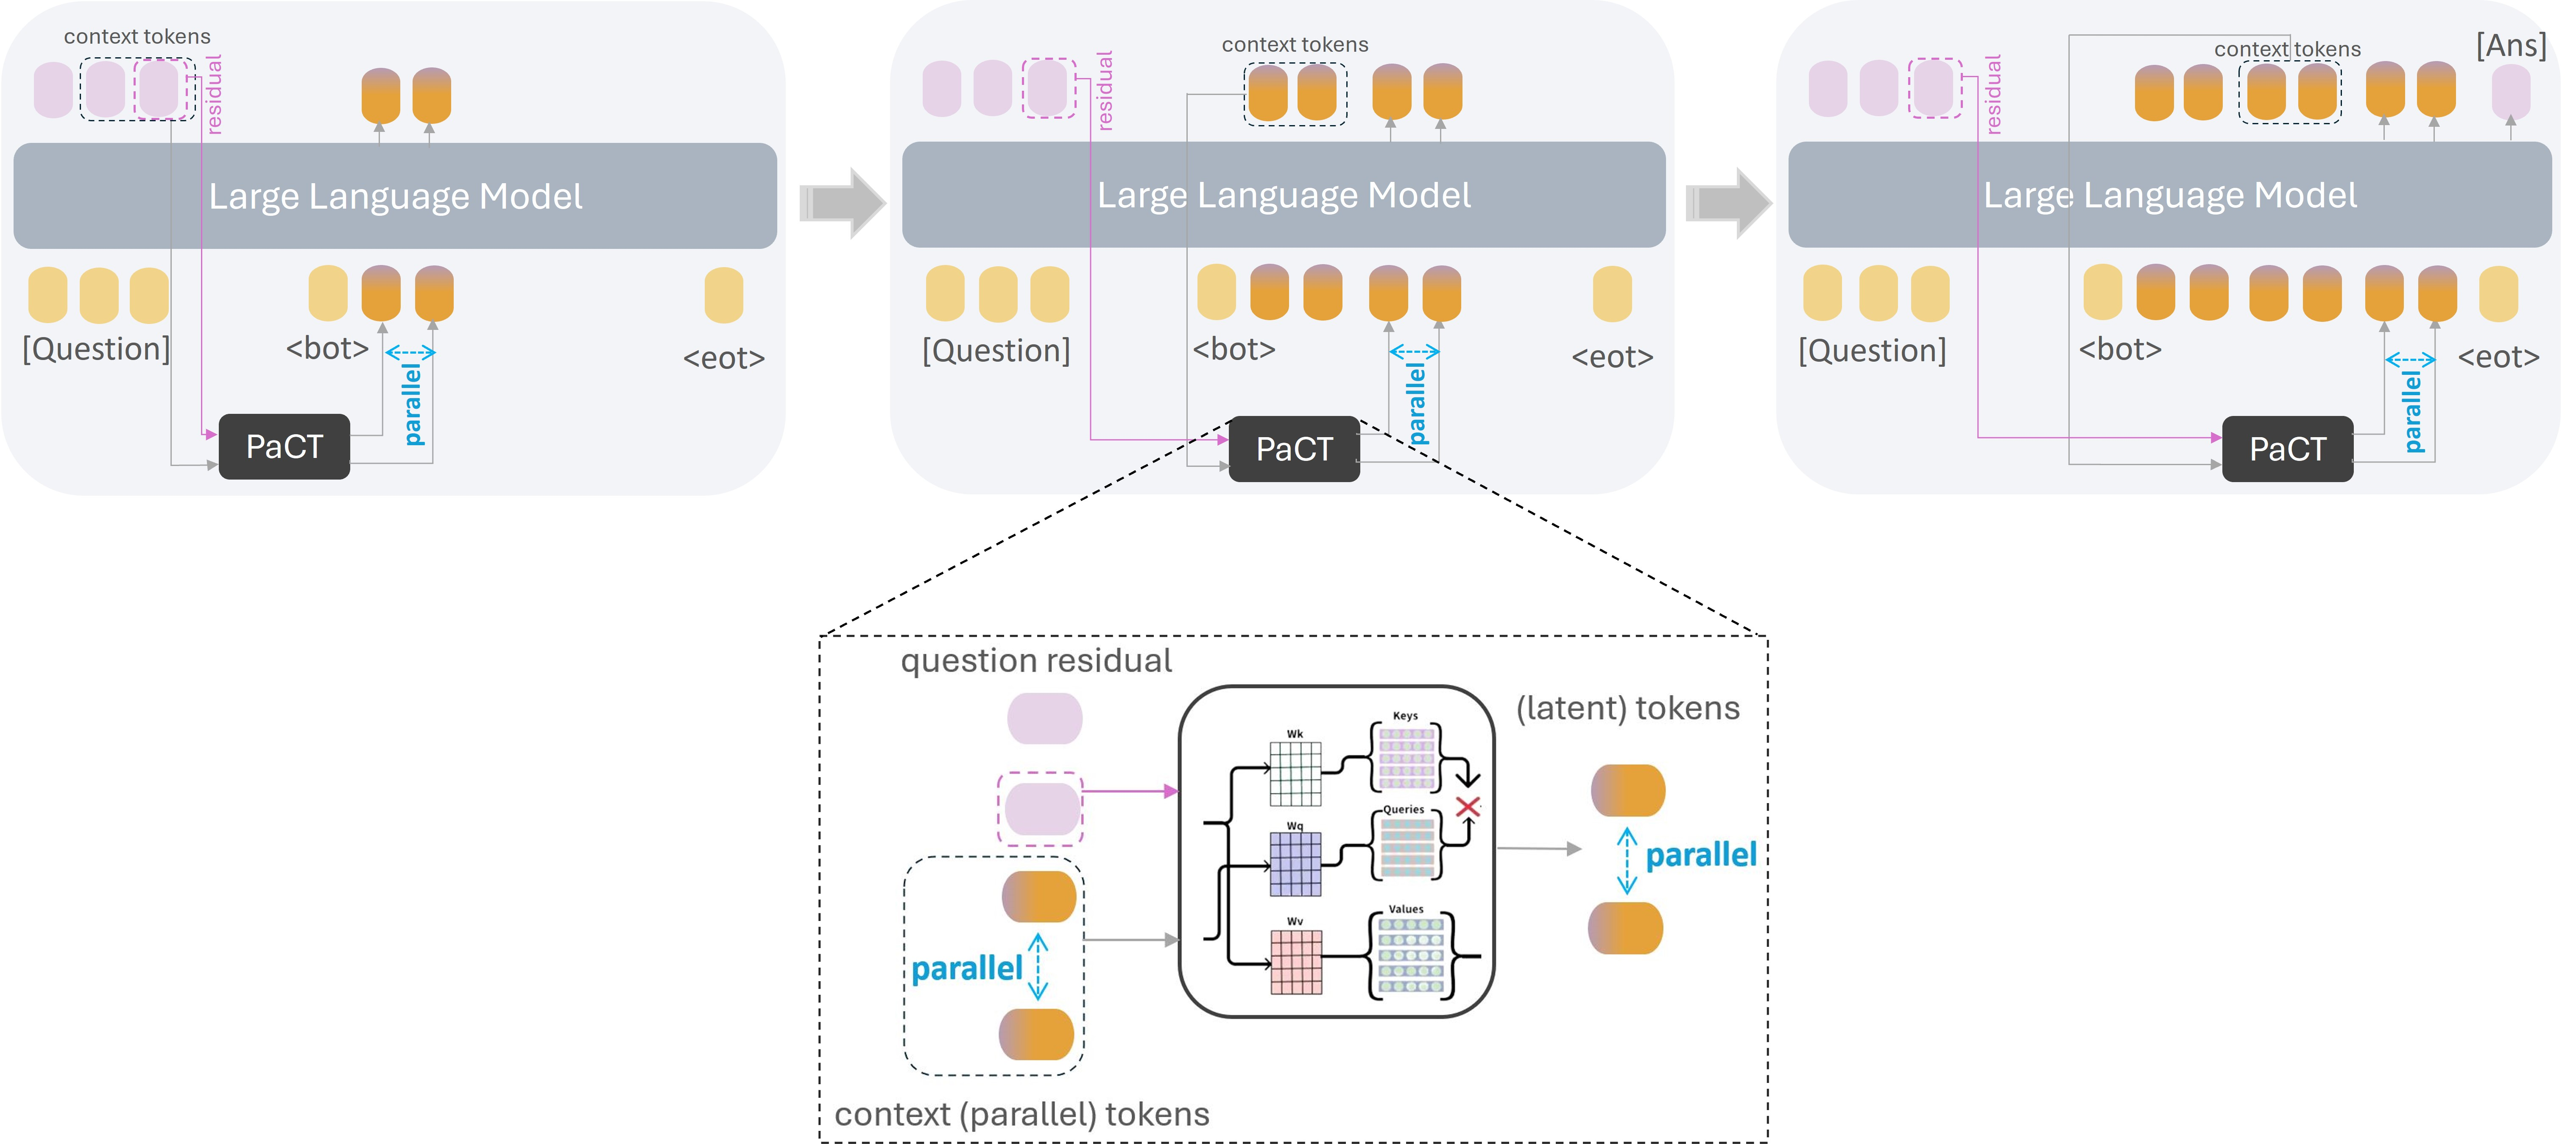
\includegraphics[width=\linewidth]{imgs/parallel_thinking_in_PaCT.jpg}
%   \caption{Parallel Continuous Thought (PaCT). At each stage, a set of latent reasoning states is synthesized in parallel from the current textual context, refined through bidirectional interaction, and used to condition subsequent autoregressive decoding.}
%   \label{fig:pact_overview}
% \end{figure*}

% PaCT replaces recurrent latent unrolling with \emph{stage-wise parallel latent reasoning}. Each stage
% constructs multiple latent reasoning states simultaneously from the current textual context, refines
% them through structured interaction, and exposes them to subsequent token decoding. Conceptually, a
% single PaCT stage proceeds as follows:

% \begin{center}
% \begin{tikzpicture}[
%     node/.style={
%         draw,
%         rounded corners,
%         inner sep=2pt,
%         font=\scriptsize
%     },
%     arrow/.style={->, thick}
% ]
% \node[node] (e) {\textbf{Text Encoding}};
% \node[node, right=4mm of e] (s) {\textbf{Latent Synthesis}};
% \node[node, right=4mm of s] (d) {\textbf{Latent Refinement}};
% \node[node, right=4mm of d] (c) {\textbf{Decoding}};

% \draw[arrow] (e) -- (s);
% \draw[arrow] (s) -- (d);
% \draw[arrow] (d) -- (c);

% \node[below=1mm of e, font=\small] {Causal};
% \node[below=1mm of s, font=\small] {Parallel};
% \node[below=1mm of d, font=\small] {Bidirectional};
% \node[below=1mm of c, font=\small] {Causal};
% \end{tikzpicture}
% \end{center}

% This structure preserves causal text processing and decoding, while enabling parallel computation
% and bidirectional interaction within each latent reasoning stage.

% \subsubsection{Latent capacity via learnable query slots}
% \label{sec:codebook}

% Let $L$ denote the number of latent reasoning states per reasoning stage. PaCT maintains a learnable set of
% query vectors
% \[
% Q = \{q_1,\dots,q_L\}, \qquad q_i \in \mathbb{R}^d,
% \]
% which define the \emph{width} of the latent reasoning set. These queries persist across examples and
% extract task-relevant summaries from the current textual context.

% \subsubsection{Parallel latent synthesis}
% \label{sec:latent_synthesis}

% Given the hidden states $H \in \mathbb{R}^{T \times d}$ of the current text prefix, PaCT synthesizes all
% latent reasoning tokens within a stage in a single cross-attention operation:
% \[
% Z = \mathrm{CrossAttn}(Q, K, V), \qquad K = V = H.
% \]
% This produces $Z \in \mathbb{R}^{L \times d}$ \emph{in parallel}. Unlike Coconut, the number of latent
% states is no longer tied to the number of sequential Transformer invocations.

% \subsubsection{Latent refinement through bidirectional interaction}
% \label{sec:latent_refinement}

% After synthesis, the latent reasoning states interact through latent-only self-attention with a
% bidirectional mask:
% \[
% Z' = \mathrm{SelfAttn}(Z).
% \]
% This interaction is confined for laten tokens within each reasoning states and does not violate causality, as
% latents do not attend to future answer tokens. Bidirectional interaction enables coordination among
% latent hypotheses within a stage, while each stage remains causally conditioned on the current text.
% Further implementation details and stability considerations are provided in Appendix~\ref{app:stability}.

% \begin{figure}[h]
%   \centering
%   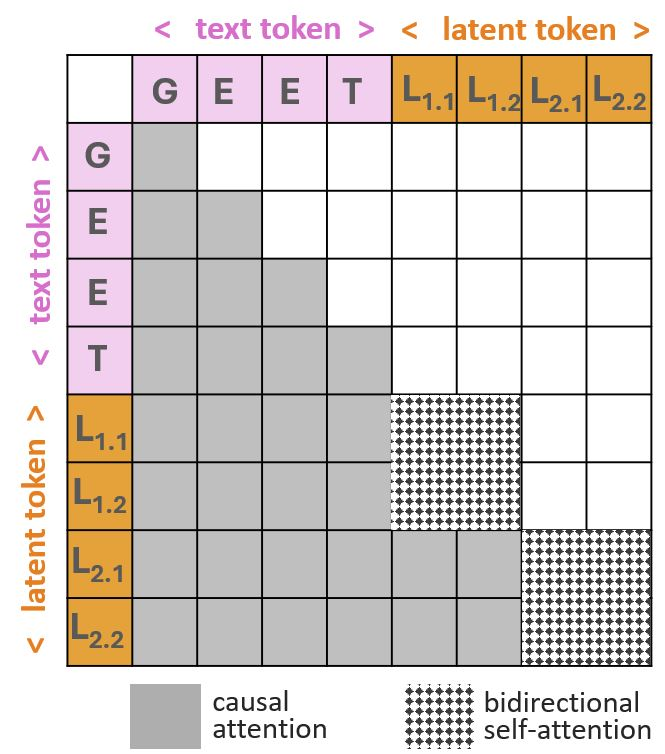
\includegraphics[width=0.6\linewidth]{imgs/bidirectional_self_attention.JPG}
%   \caption{Bidirectional interaction among latent reasoning states within a stage, while preserving causal text decoding.}
%   \label{fig:latent_attention}
% \end{figure}

% \subsubsection{Conditioning decoding on latents}
% \label{sec:conditioning}

% Autoregressive decoding is conditioned on the latent reasoning states through a causal interface:
% answer tokens may attend to both prior text tokens and all latent states produced in previous stages.
% We implement this by concatenating latent states into the attention context and adding a cross-attention
% pathway from text representations to latent keys and values. The resulting factorization is
% \[
% p(a \mid q) \;\approx\; p(a \mid q,\; Z'^{(1:S)}),
% \]
% where $Z'^{(1:S)}$ denotes the continuous latent reasoning tokens across $S$ stages. The precise attention masking
% rules are given in Appendix~\ref{app:masking}.

% \subsubsection{Multi-stage latent reasoning}
% \label{sec:stages}

% PaCT applies the above procedure for $S$ stages, yielding two scaling axes: width $L$ (latent states
% per stage) and depth $S$ (number of stages). Increasing depth introduces additional reasoning steps
% without increasing latent width or serial dependency. Empirically, we find that scaling depth is more
% effective than scaling width, consistent with latent similarity analyses presented later.

% \subsection{Training}
% \label{sec:training}

% PaCT is trained using a curriculum similar to Coconut~\cite{hao2024training}, which progressively
% replaces supervised text CoT tokens with continuous latent states. At curriculum stage $s$, the first
% $m_s$ rationale tokens are replaced by $S_s$ latent stages, while the remaining rationale (if any)
% and the answer remain as language tokens.

% Training minimizes the standard next-token prediction loss on text tokens, with the loss masked on
% latent positions:
% \[
% \mathcal{L}(\theta) = -\sum_{t \in \mathcal{I}_{\text{text}}}
% \log p_\theta(x_t \mid x_{<t}, Z'^{(1:S)}).
% \]
% The full training algorithm is provided in Appendix~\ref{app:algorithm}.

% \subsection{Computational analysis}
% \label{sec:complexity}

% Efficiency is governed by serial depth, i.e., the length of the critical path that cannot be
% parallelized. Let $T$ be the number of text decoding steps and $n_{\text{lat}}$ the total number of
% latent states.

% In Coconut, latent states are generated recurrently, yielding
% \[
% D_{\text{seq}}^{\textsc{Coconut}} = T + n_{\text{lat}}.
% \]
% In PaCT, $L$ latent states are generated in parallel per stage, and only the number of stages $S$
% contributes to serial depth:
% \[
% D_{\text{seq}}^{\textsc{PaCT}} = T + S, \qquad n_{\text{lat}} = S L.
% \]
% Thus, for a fixed latent budget, PaCT reduces latent-induced serial depth by a factor of $L$. PaCT
% shifts computation from serialized Transformer invocations to parallel attention and matrix
% multiplications, enabling substantially improved hardware utilization.
\section{Methodology}
\label{sec:method}

\subsection{Objective and problem formulation}
\label{sec:objective}

We study supervised reasoning tasks where each training example consists of a question $q$,
an optional chain-of-thought expressed as text tokens $r = (r_1,\dots,r_M)$, and a final answer
$a = (a_1,\dots,a_N)$. The full textual sequence is
\[
y \;=\; [\,q \,;\, r \,;\, a\,].
\]
A standard causal language model (LM) parameterized by $\theta$ learns $p_\theta(y)$ via maximum
likelihood training.

\paragraph{Goal.}
Our goal is to enable multi-step reasoning using \emph{continuous} internal representations while
preserving standard autoregressive decoding of the answer, and crucially, avoiding the \emph{serial}
compute bottleneck that arises when continuous reasoning is implemented through recurrent latent
unrolling.
\vspace{-3mm}
\paragraph{Key bottleneck.}
% Chain of Continuous Thought (Coconut)~\cite{hao2024training} replaces segments of textual chain-of-thought
% (CoT) tokens with continuous latent states, but generates these latent states \emph{sequentially} by
% feeding the previous hidden state back as the next input embedding. This induces a recurrent dependency
% across latent steps, causing serial depth to grow linearly with the number of latent states and limiting
% hardware parallelism. Moreover, each latent state must implicitly carry forward information from
% earlier steps, reducing representational separation across reasoning stages.
Chain of Continuous Thought (Coconut)~\cite{hao2024training} replaces segments of textual chain-of-thought
(CoT) tokens with continuous latent states, but generates these states \emph{sequentially} by feeding the
previous hidden state back as the next input embedding. This induces recurrent dependencies across latent
steps, causing serial depth to grow linearly with the number of latent states, limiting hardware
parallelism, and reducing representational separation across reasoning stages.

\vspace{-3mm}

\paragraph{Hypothesis.}
We hypothesize that the benefits of continuous latent reasoning do not require recurrent latent
unrolling. Instead, effective reasoning can be achieved by (i) synthesizing a \emph{set} of latent
reasoning states in parallel from the current textual context, (ii) allowing structured interaction
\emph{within} each reasoning stage, and (iii) conditioning autoregressive decoding on these states
through a causal interface, without directly propagating latent states across stages.

\subsection{Preliminaries: causal LMs and Coconut-style latent replacement}
\label{sec:prelims}

A causal Transformer LM maps token prefixes $x_{\le t}$ to hidden states
$H_t \in \mathbb{R}^{t \times d}$ and predicts the next token via
\[
p_\theta(x_{t+1}\mid x_{\le t}) = \mathrm{softmax}(W h_t).
\]

Coconut~\cite{hao2024training} replaces a prefix of textual CoT tokens with continuous latent states
that are not decoded as language. During this latent phase, each latent state is generated by feeding
the previous hidden state as the next input embedding, creating a recurrent unrolling within the
Transformer, reinstating an RNN-like bottleneck within an otherwise parallel architecture.

\subsection{Parallel Continuous Thought (PaCT)}
\label{sec:pact}

\begin{figure*}[t]
  \centering
  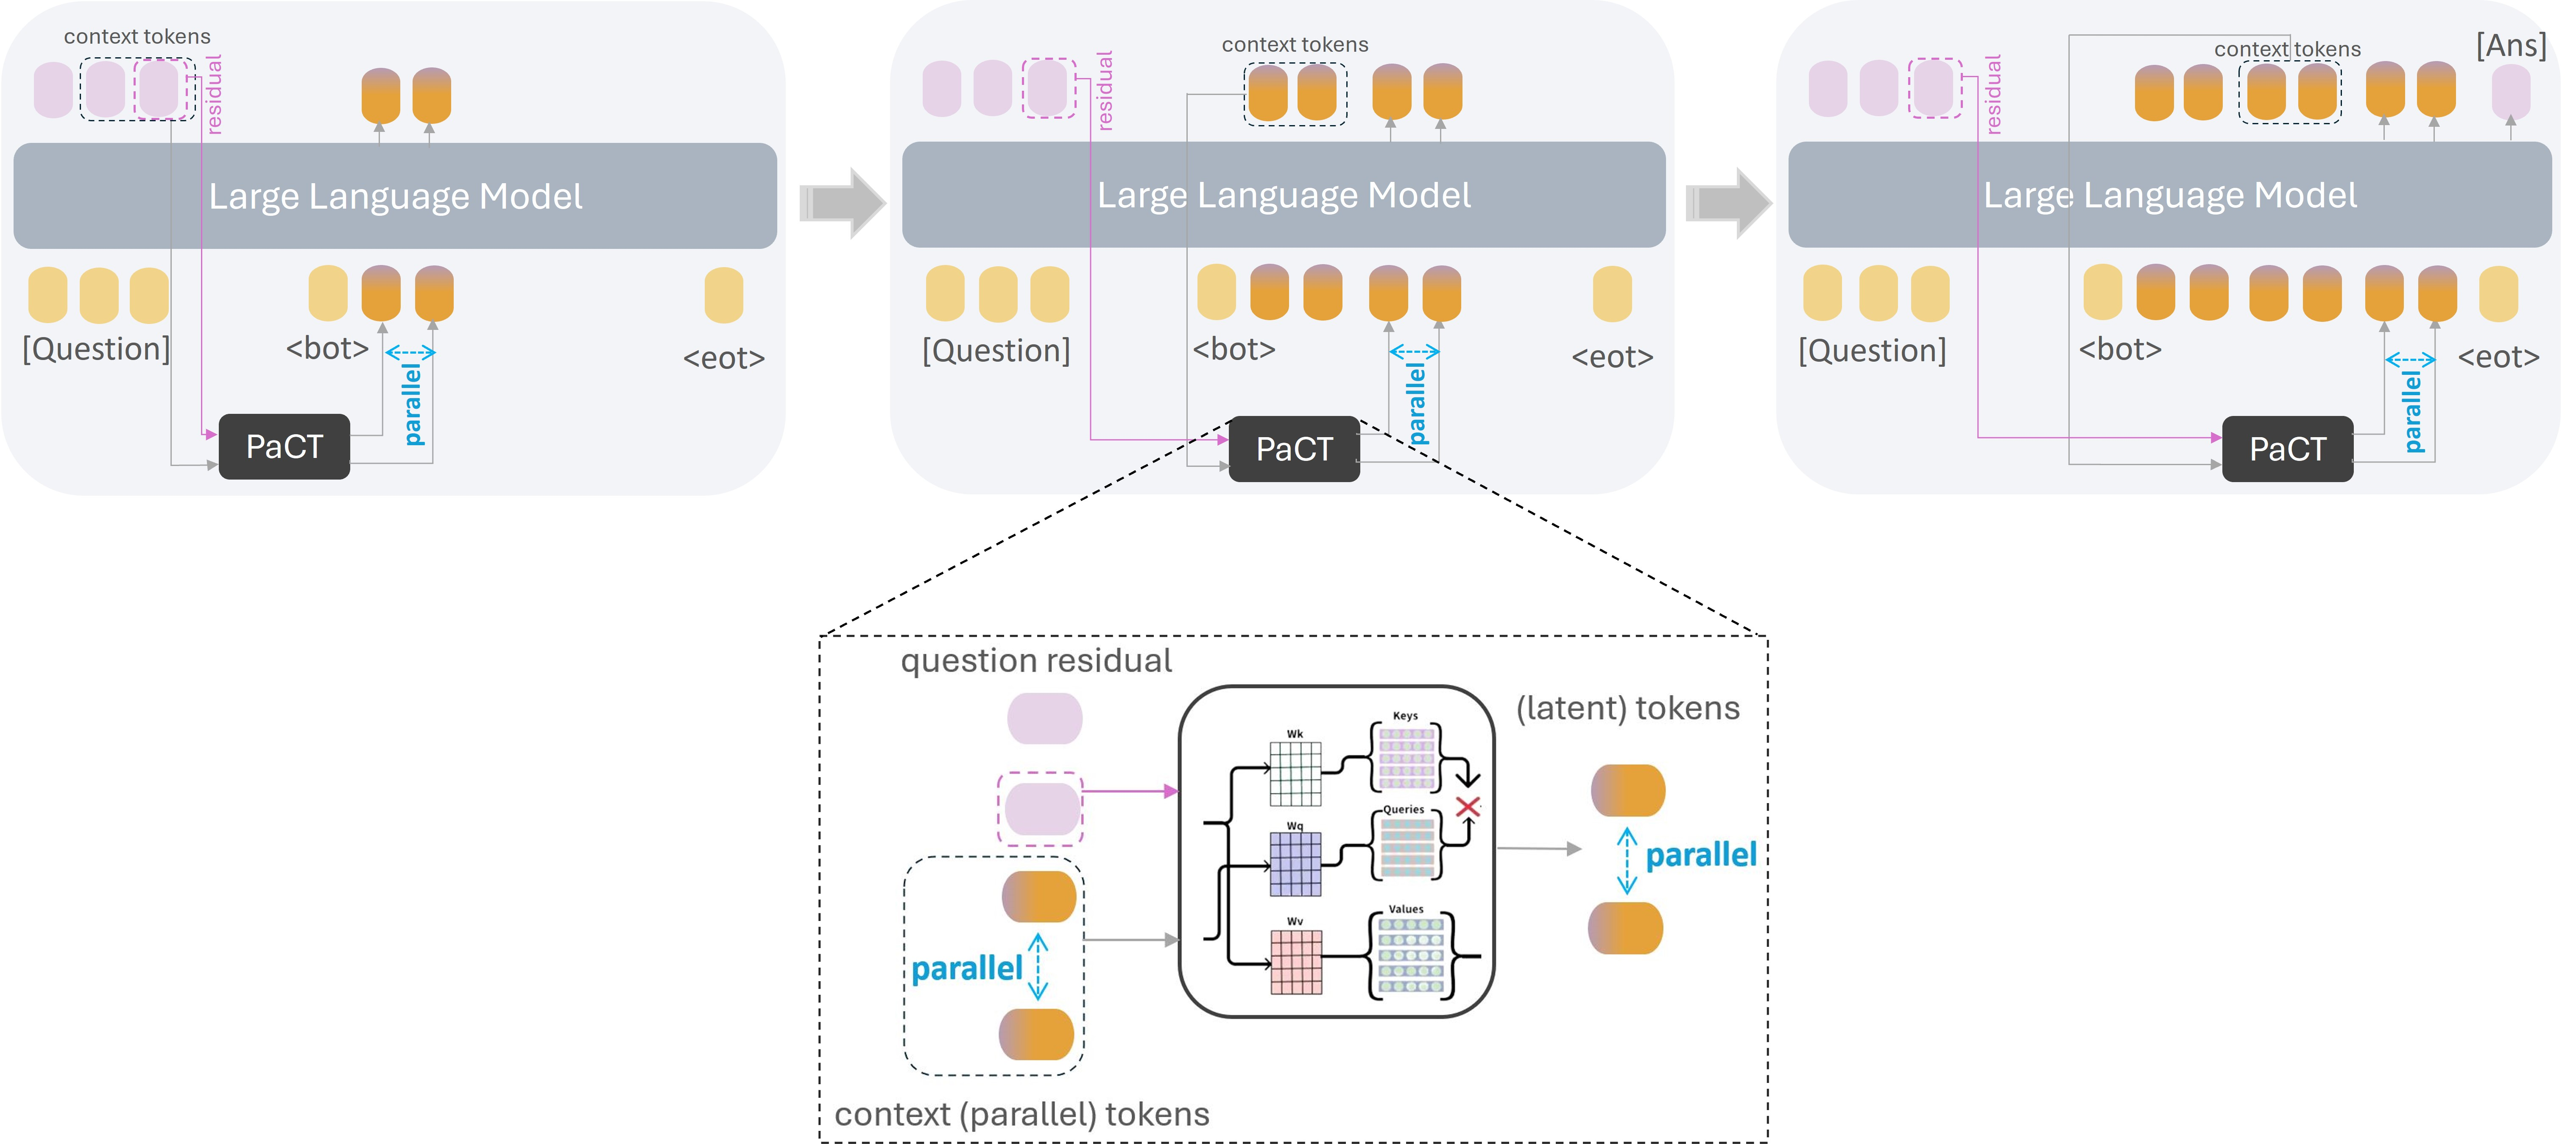
\includegraphics[width=0.9\linewidth]{imgs/parallel_thinking_in_PaCT.jpg}
  \caption{\textbf{Parallel Continuous Thought (PaCT).} At each reasoning stage, a set of latent reasoning states
  is synthesized in parallel from the current textual context, refined through bidirectional interaction,
  and used to condition subsequent autoregressive decoding.}
  \label{fig:pact_overview}
\end{figure*}

PaCT replaces recurrent latent unrolling with \emph{stage-wise parallel latent reasoning}. Rather than
propagating latent states across time, PaCT organizes reasoning into a sequence of stages. Each stage
constructs a fresh set of latent reasoning states directly from the current textual context, allows
structured interaction among them, and then exposes them to subsequent decoding. Importantly, latent
states do not directly transform or depend on latent states from earlier stages. Parallelism in PaCT arises as a consequence of stage-wise latent resynthesis: since latent reasoning states are re-synthesized from the current context rather than propagated from previous states, they can be generated simultaneously within each stage.

Conceptually, a single PaCT reasoning stage proceeds as follows:

\begin{center}
\begin{tikzpicture}[
    node/.style={
        draw,
        rounded corners,
        inner sep=2pt,
        font=\scriptsize
    },
    arrow/.style={->, thick}
]
\node[node] (e) {\textbf{Text Encoding}};
\node[node, right=4mm of e] (s) {\textbf{Latent Synthesis}};
\node[node, right=4mm of s] (d) {\textbf{Latent Refinement}};
\node[node, right=4mm of d] (c) {\textbf{Decoding}};

\draw[arrow] (e) -- (s);
\draw[arrow] (s) -- (d);
\draw[arrow] (d) -- (c);

\node[below=1mm of e, font=\small] {Causal};
\node[below=1mm of s, font=\small] {Parallel};
\node[below=1mm of d, font=\small] {Bidirectional};
\node[below=1mm of c, font=\small] {Causal};
\end{tikzpicture}
\end{center}

This structure preserves causal text processing and decoding, while enabling parallel computation and
bidirectional interaction \emph{within} each reasoning stage.

\subsubsection{Latent capacity via learnable query slots}
\label{sec:codebook}

Let $L$ denote the number of latent reasoning states per stage. PaCT maintains a learnable set of query
vectors
\[
Q = \{q_1,\dots,q_L\}, \qquad q_i \in \mathbb{R}^d,
\]
which define the \emph{width} of the latent reasoning set. These queries persist across examples and
extract task-relevant summaries from the current textual context. We use the term \emph{latent reasoning
state} to denote a continuous hidden vector that participates in reasoning but is never decoded as
language.

\subsubsection{Parallel latent synthesis}
\label{sec:latent_synthesis}

Given the hidden states $H \in \mathbb{R}^{T \times d}$ of the current text prefix, PaCT synthesizes all
latent reasoning states for a stage in a single cross-attention operation:
\[
Z = \mathrm{CrossAttn}(Q, K, V), \qquad K = V = H.
\]
This produces $Z \in \mathbb{R}^{L \times d}$ \emph{in parallel}. In contrast to Coconut, the number of
latent reasoning states is no longer tied to the number of sequential Transformer invocations, and no
latent state depends on another for its construction.

\subsubsection{Latent refinement within a stage}
\label{sec:latent_refinement}

After synthesis, latent reasoning states interact \emph{only within the same stage} through latent-only
self-attention with a bidirectional mask:
\[
Z' = \mathrm{SelfAttn}(Z).
\]
This bidirectional interaction enables coordination among latent hypotheses within a stage. It does
not violate causality, as latent states do not attend to future answer tokens, and text tokens do not
attend to latent states. No bidirectional interaction occurs across different stages.

\begin{figure}[h]
  \centering
  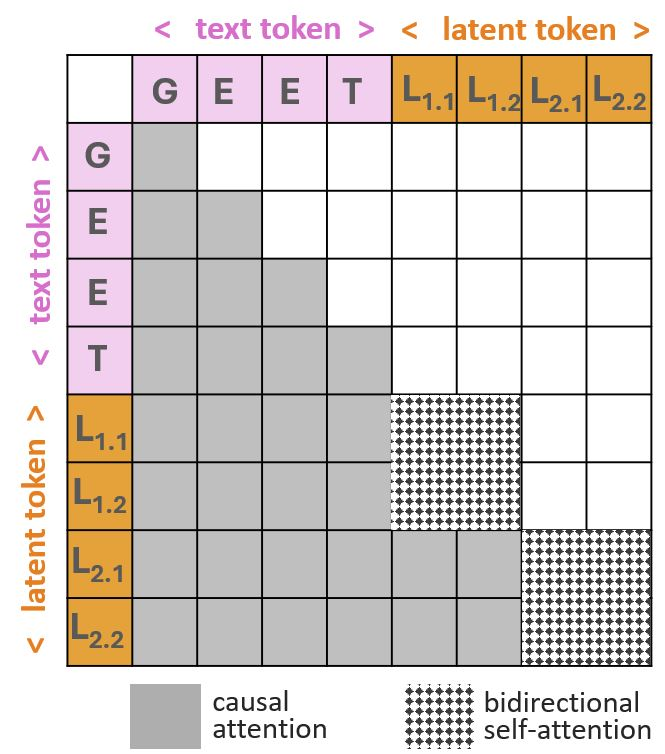
\includegraphics[width=0.4\linewidth]{imgs/bidirectional_self_attention.JPG}
  \caption{Bidirectional interaction among latent reasoning states within a single stage, while
  preserving causal text decoding.}
  \label{fig:latent_attention}
\end{figure}

\subsubsection{Conditioning decoding on latent reasoning states}
\label{sec:conditioning}

Autoregressive decoding is conditioned on latent reasoning states through a causal interface. Answer
tokens may attend to both prior text tokens and all latent reasoning states produced in \emph{earlier
stages}. Latent states themselves never attend to answer tokens.

Concretely, we concatenate latent reasoning states into the attention context and add a cross-attention
pathway from text representations to latent keys and values. This realizes the factorization
\[
p(a \mid q) \;\approx\; p(a \mid q,\; Z'^{(1:S)}),
\]
where $Z'^{(1:S)}$ denotes the latent reasoning states across $S$ stages. The attention masking rules
that enforce this causal structure are detailed in Appendix~\ref{app:masking}.

\subsubsection{Multi-stage latent reasoning}
\label{sec:stages}

PaCT applies the above procedure for $S$ reasoning stages. All latent states within a stage are synthesized
simultaneously from a restricted window of the most recent $k$ positions in the sequence, which may include
text tokens, latent states from earlier stages, or both. The window size $k$ is a fixed hyperparameter,
with its impact analyzed in Table~\ref{tab:gpt2_gsm8k_context} and Figure~\ref{fig:attention_heatmap}.
This yields two independent scaling axes: width $L$ (latent states per stage) and depth $S$ (number of
reasoning stages). Increasing depth adds reasoning capacity without increasing latent width or serial
dependency.


\subsection{Training}
\label{sec:training}

PaCT is trained using a curriculum similar to Coconut~\cite{hao2024training}, which progressively
replaces steps of CoT with continuous latent reasoning tokens. 
At curriculum stage $s$, a prefix of the textual chain-of-thought is replaced by $s$ latent reasoning stages, each consisting of $L$ latent reasoning states synthesized in parallel. The remaining CoT tokens (if any) and the answer remain as language tokens. This curriculum stabilizes optimization compared to training directly from $(q, a)$ pairs.

Training minimizes the standard next-token prediction loss on text tokens, with the loss masked on
latent positions:
\[
\mathcal{L}(\theta) = -\sum_{t \in \mathcal{I}_{\text{text}}}
\log p_\theta(x_t \mid x_{<t}, Z'^{(1:S)}).
\]
The full training algorithm is provided in Appendix~\ref{app:algorithm}.

\subsection{Computational analysis}
\label{sec:complexity}

Efficiency is governed by serial depth, i.e., the length of the critical path that cannot be
parallelized. Let $T$ be the number of text decoding steps and $n_{\text{lat}}$ the total number of
latent reasoning states.

In Coconut, latent reasoning states are generated recurrently, yielding
\[
D_{\text{seq}}^{\textsc{Coconut}} = T + n_{\text{lat}}.
\]
In PaCT, $L$ latent reasoning states are generated in parallel per stage, and only the number of
stages $S$ contributes to serial depth:
\[
D_{\text{seq}}^{\textsc{PaCT}} = T + S, \qquad n_{\text{lat}} = S L.
\]
Thus, for a fixed latent budget, PaCT reduces latent-induced serial depth by a factor of $L$. PaCT
shifts computation from the critical path to parallel attention and matrix multiplications, which
modern accelerators can efficiently amortize.

